\section{Изисквания към продукта}
Продуктът трябва да осъществява връзката между работници, които желаят еднодневна, бърза работа и работодатели, които имат нужда от помощ с всякакъв вид битова дейност. Начинът, по който това трябва да се осъществи, е чрез обяви, които могат да се качват в приложението от работодателите. Те трябва да съдържат нужната информация за работата като град, предлаганата сума, нужният брой работници и описание на дейността, която трябва да се извърши. Потенциалните работниците трябва да имат възможност да изберат от всички обяви най-желаната и удобна за тях. За да се улесни търсенето, трябва да може да се филтрира чрез всичките полета в обявата, което би улеснило откриването на най-подходящата за тях работа. След като направят своят избор те трябва да заявят желание за участие чрез подаване на заявление. Работодателят ще има възможност да избере предпочитания от него работник или работници. За да може той да направи най-добрия избор, той ще има достъп до обратните връзки от предишни техни работодатели. Приложението дава възможност на работодателя да отбележи кога е стартирало реалното изпълнение на дейността и кои от приетите от него работници са се явили. Ако работник е приет от работодател, но не се е явил на посочените от него място и час за извършване на дейността, това би понижило неговия рейтинг. Работодателят ще има възможността да отбележи края на дейността, след което да остави своята обратна връзка за работата на всеки един от работниците.

\section{Използвани технологии}

    \subsection{IntelliJ}
    
    
    \begin{figure}[h]
        \centering
        
\includegraphics[scale=.06]{images/intellij.png}
        \caption{IntelliJ Лого}
        \label{fig:intelliJ}
    \end{figure}
    
    IntelliJ е среда за разработка на софтуер с Java създадена от JetBrains. Използвайки тази среда е улеснено създаването на проекта заради характеристики, като  завършеност на кода чрез анализ на контекста, навигация на кода, която позволява да се направи клас или декларация в кода директно, да го преработи и да предостави възможности за поправяне на несъответствия чрез предложения. Според статията на Андрей Соинцев\parencite{IntelliJ}, IntelliJ е по-добра среда за разработка на Java софтуерни продукти от Eclipse възлагайки следните точки:
    \begin{itemize}
        \item Повече възможности при дебъгване
            При дебъгване на софтуер, IntelliJ възлага много повече нужна информация и откриването на стойностите на желаните параметри е лесно и интуитивно.
        \item Интелигентен autocomplete
            IntelliJ има способността да разбира от контекста, в който кодът се намира и успява да спомага в процеса на писането му. Autocomplete е основната услуга, която разграничава развойна среда от текстов редактор и поради тази причина доброто му осъществяване е от голямо значение.
        \item Големи възможности при рефакториране
            Рефакторирането е част от всяка развойна среда, но IntelliJ отново успява да го осъществи по "интелигентен" начин. Средата успява да определи контекста на това, което програмистът се опитва да рефакторира и улеснява работата му значително. Аз лично съм се възползвал от тези услуги множество пъти по време на изработване на дипломнта работа.
    \end{itemize}
    
    \subsection{Kotlin}
    \begin{figure}[ht]
        \centering
        
\includegraphics[scale=.4]{images/kotlin.png}
        \caption{Kotlin Лого}
        \label{fig:Kotlin}
    \end{figure}
    Котлин е език за програмиране, който излиза за публично използване през 2012 година, но добива популярност през 2016 с излизането на Котлин 1.0. Езикът е създаден от JetBrains(създателите и на IntelliJ) и е създаден да работи изцяло с и вместо Java, използвайки основните библютеки на предшественика си. Плюсовете за използване на Kotlin вместо Java са много и Магнус Винтер излага част от тях в статията си "Why you should tottaly switch to Kotlin"\parencite{Kotlin}:
    \begin{itemize}
        \item Съвместимост с Java
        
        
            Kotlin позволява съвсем свободното писане на Java код съвместно с него. Той може да замести или да обогати вече написан Java код. Това значи, че всички възможности и архитектури, които Java предоставя, са достъпни и от Kotlin.
        \item Познат синтаксис
        
        
            Kotlin е подобен по синтаксис на повечетео обектно-ориентирани езици. Поради тази причина научването и използването му е тривиално. Kotlin все пак принася и новости като val и var деклараторите за променливи, но те също единствено спомагат на работата с езика.
        \item Интерполация на текст
        
        
            Езикът предоставя лесна обработка на променливи в текст.
        \item Извод за типа променлива
        
        
            За разлика от предшественика си, Kotlin има способността сам да прави изводи за типа променливи, които се създават и използват.
        \item Аргументи по подразбиране
        
            При избиране на аргументите, езикът предлага задаванет на стойността им по подразбиране, елиминрайки нуждата от създаването на множествно методи.
        \item Именувани аргументи
        
        
            Заедно с аргументите по подразбиране се елеминира нуждата от използването на билдер модела.
        \item When функцията
        
        
            Switch case е заменен с много по-удобната when функция.
        \item Data класът
        
        
            В Котлин е възможно създаването на клас от тип data. Това автоматично създава toString(), equals(), hashCode() и copy(), което отстранява кода, който иначе би се налагало да се пише на Java.
        \item Extension функции
        
        
            Котлин има възможността да се пишат extension функции към някой клас. По този наичн би могло да се добавят нужни функции към стари Java библиотеки.
        \item Обезопасяване от null
        
        
            В Java при инстанцирането на обект се задава неговият клас. Но това не осигурява, че стойноста на обекта или променливата няма да бъде null. Котлин отстранява този проблем като прави разлика между обекти, които биха могли да бъдат null и обекти, които не трябва да могат. Това се прави чрез изписването на името на класа и добавянето на ``?'' в края на класа.
            Пр. val age: Int?
    \end{itemize}
    
    \subsection{Spring}
    
    \begin{figure}[h]
        \centering
        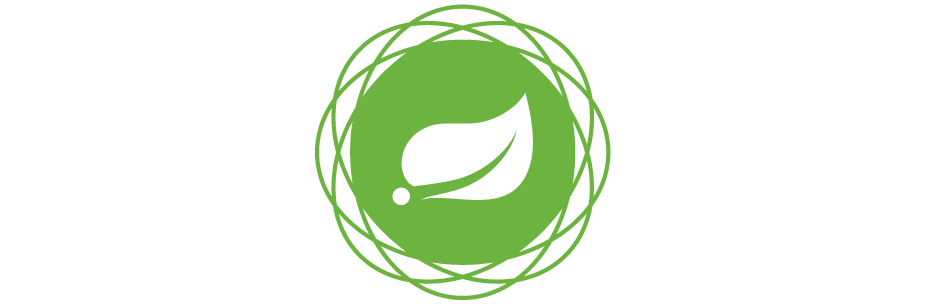
\includegraphics[scale=0.5]{images/spring-framework.png}
        \caption{Spring Лого}
        \label{fig:intellij_logo}
    \end{figure}
    Spring е технологична рамка, която улеснява свързването между множество компоненти чрез IoC(Inversion of Control) и Dependency Injection. Inversion of Control е принцип в програмирането, който позволява обръщането на последователността на изпълнението на отделни заявки. Използвайки IoC е възможно да се раздели програмния код на отделни компоненти, които изпълняват своите заявки спрямо дефинираната последователност на кода. Това позволява лесното разширяване на програмата, когато има нужда от това. 
    
    Dependency Injection е принцип, който се използва за снабдяването на отделните компоненти с техните зависимости. Spring е най-известната и използвана технологична рамка за Java проекти. В контекста на уеб апликации Spring е перфектната технология за създаването на бек енда на Jobche. Използвайки различните технологии, които Spring предоставя, създаването на системата става лесно и интуитивно.
    
        \subsubsection{Spring MVC}
            Spring MVC(Model-View-Controller) е технологична рамка и част от Spring, която предоставя лесно имплементиране на Model-View-Controller модела, чиято цел е цялостното ограничаване между различните компоненти в програмния код. Това е основната технологична рамка, която поема грижата за заявките, тяхното изпълнение и връщането на съответния отговор.
        
        \subsubsection{Spring Data}
            Spring Data е модел за лесно работене с бази данни. Технологията предоставя множестно компоненти за работене с бази данни, но основният, който се използва в проекта е Spring Data JPA. Spring Data JPA e програмна рамка за създаване и изпълняване на команди върху хранилища създадени на принципа JPA.
        
        \subsubsection{Spring Security}
            Spring Security е технологична рамка за защитаване на проекти създадени със Spring. Тя позволява контрол върху заверяването и упълномощаване на всяка заявка. В проекта е използван за създаване на Basic Authentication на всяка заявка.
            
            \subsubsection{Spring Boot}
        Spring Boot \textbf{не е} технологична рамка, а начин за изработване на Spring проекти. Чрез него лесно можем да стартираме Spring проект, тъй като ни предоставя вграден сървлет. Има множество библиотеки, които Spring Boot предоставя за лесното започване и създаване на софтуер чрез тази технологична рамка. На https://start.spring.io/ може автоматинчо да се създаде Spring Boot проект като имаме опцията да изберем зависимостите, които желаем да използваме. 
    
    \subsection{JUnit5}
    \begin{figure}[h]
        \centering
        
\includegraphics{images/junit5.png}
        \caption{JUnit5 Лого}
        \label{fig:junit5_logo}
    \end{figure}
    
    JUnit е технологична рамка за създаване на тестове върху отделни компоненти и класове, използвайки езици от семейството на Java. В проекта това е основната използвана технология за структурирането и създаването на тестове. Презентацията на Филип Хауер е основната ми мотивация за използването на именно тези технологии за създаването на тестове\parencite{Testing}. В презентацията си той представя JUnit5 като най-добрата технологична рамка за писане на тестове с Kotlin. Поради разликите на Kotlin с Java възникват проблеми при използването на по-стари версии на JUnit, тъй като е написан с идеята да се използва в тандем с Java. Но JUnit5 е написан взимайки предвид концепции от Kotlin. Поради тази причина JUnit5 е перфектният избор за създаване на тестове в този проект.
    
        \subsubsection{AssertJ}
        AssertJ е библиотека за създаване на проверки за Java. Библиотеката е най-често използвана и най-добре пригодена за използване заедно с JUnit. В презентацията си Филип Хауер набляга върху огромния брой възможни проверки, които AssertJ предоставя. Именно поради тези причина аз избрах нея за библиотеката за създаване на проверки в проекта.
        
        \subsubsection{MockK}
        MockK e библиотека за създаване на Mock обекти при писането на тестови код. Мокването е важна концепция в света на тестовете и избора на правилна библиотека играе важна роля за цялостното създаване на тестове. Изборът ми на MockK като библиотека за мокване в проекта идва пак от презентацията на Филип Хауер.
    
    \subsection{Swagger}
    
    \begin{figure}[h]
        \centering
        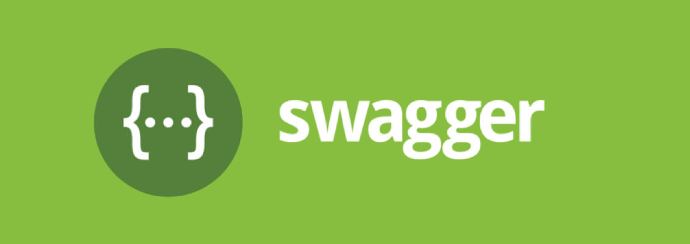
\includegraphics[scale=.5]{images/Swagger.png}
        \caption{Swagger Лого}
        \label{fig:swagger_logo}
    \end{figure}
    
    Swagger е технологична рамка, която помага на програмистта да създаде дизайна и документацията на своя RESTful уеб продукт. Добрата документация на бекенда е важна за лесното й използване от клиентски приложения. Тъй като бекенда е използван от андроид приложение, Swagger много спомага за лесното документиране на всяка крайна точка на бек енд-а. За целта е използван специфично Swagger UI за Spring приложение, имплементирано от Springfox. 
    
\section{Основен алгоритъм}
\begin{figure}[h]
    \centering
    \makebox[\textwidth][c]{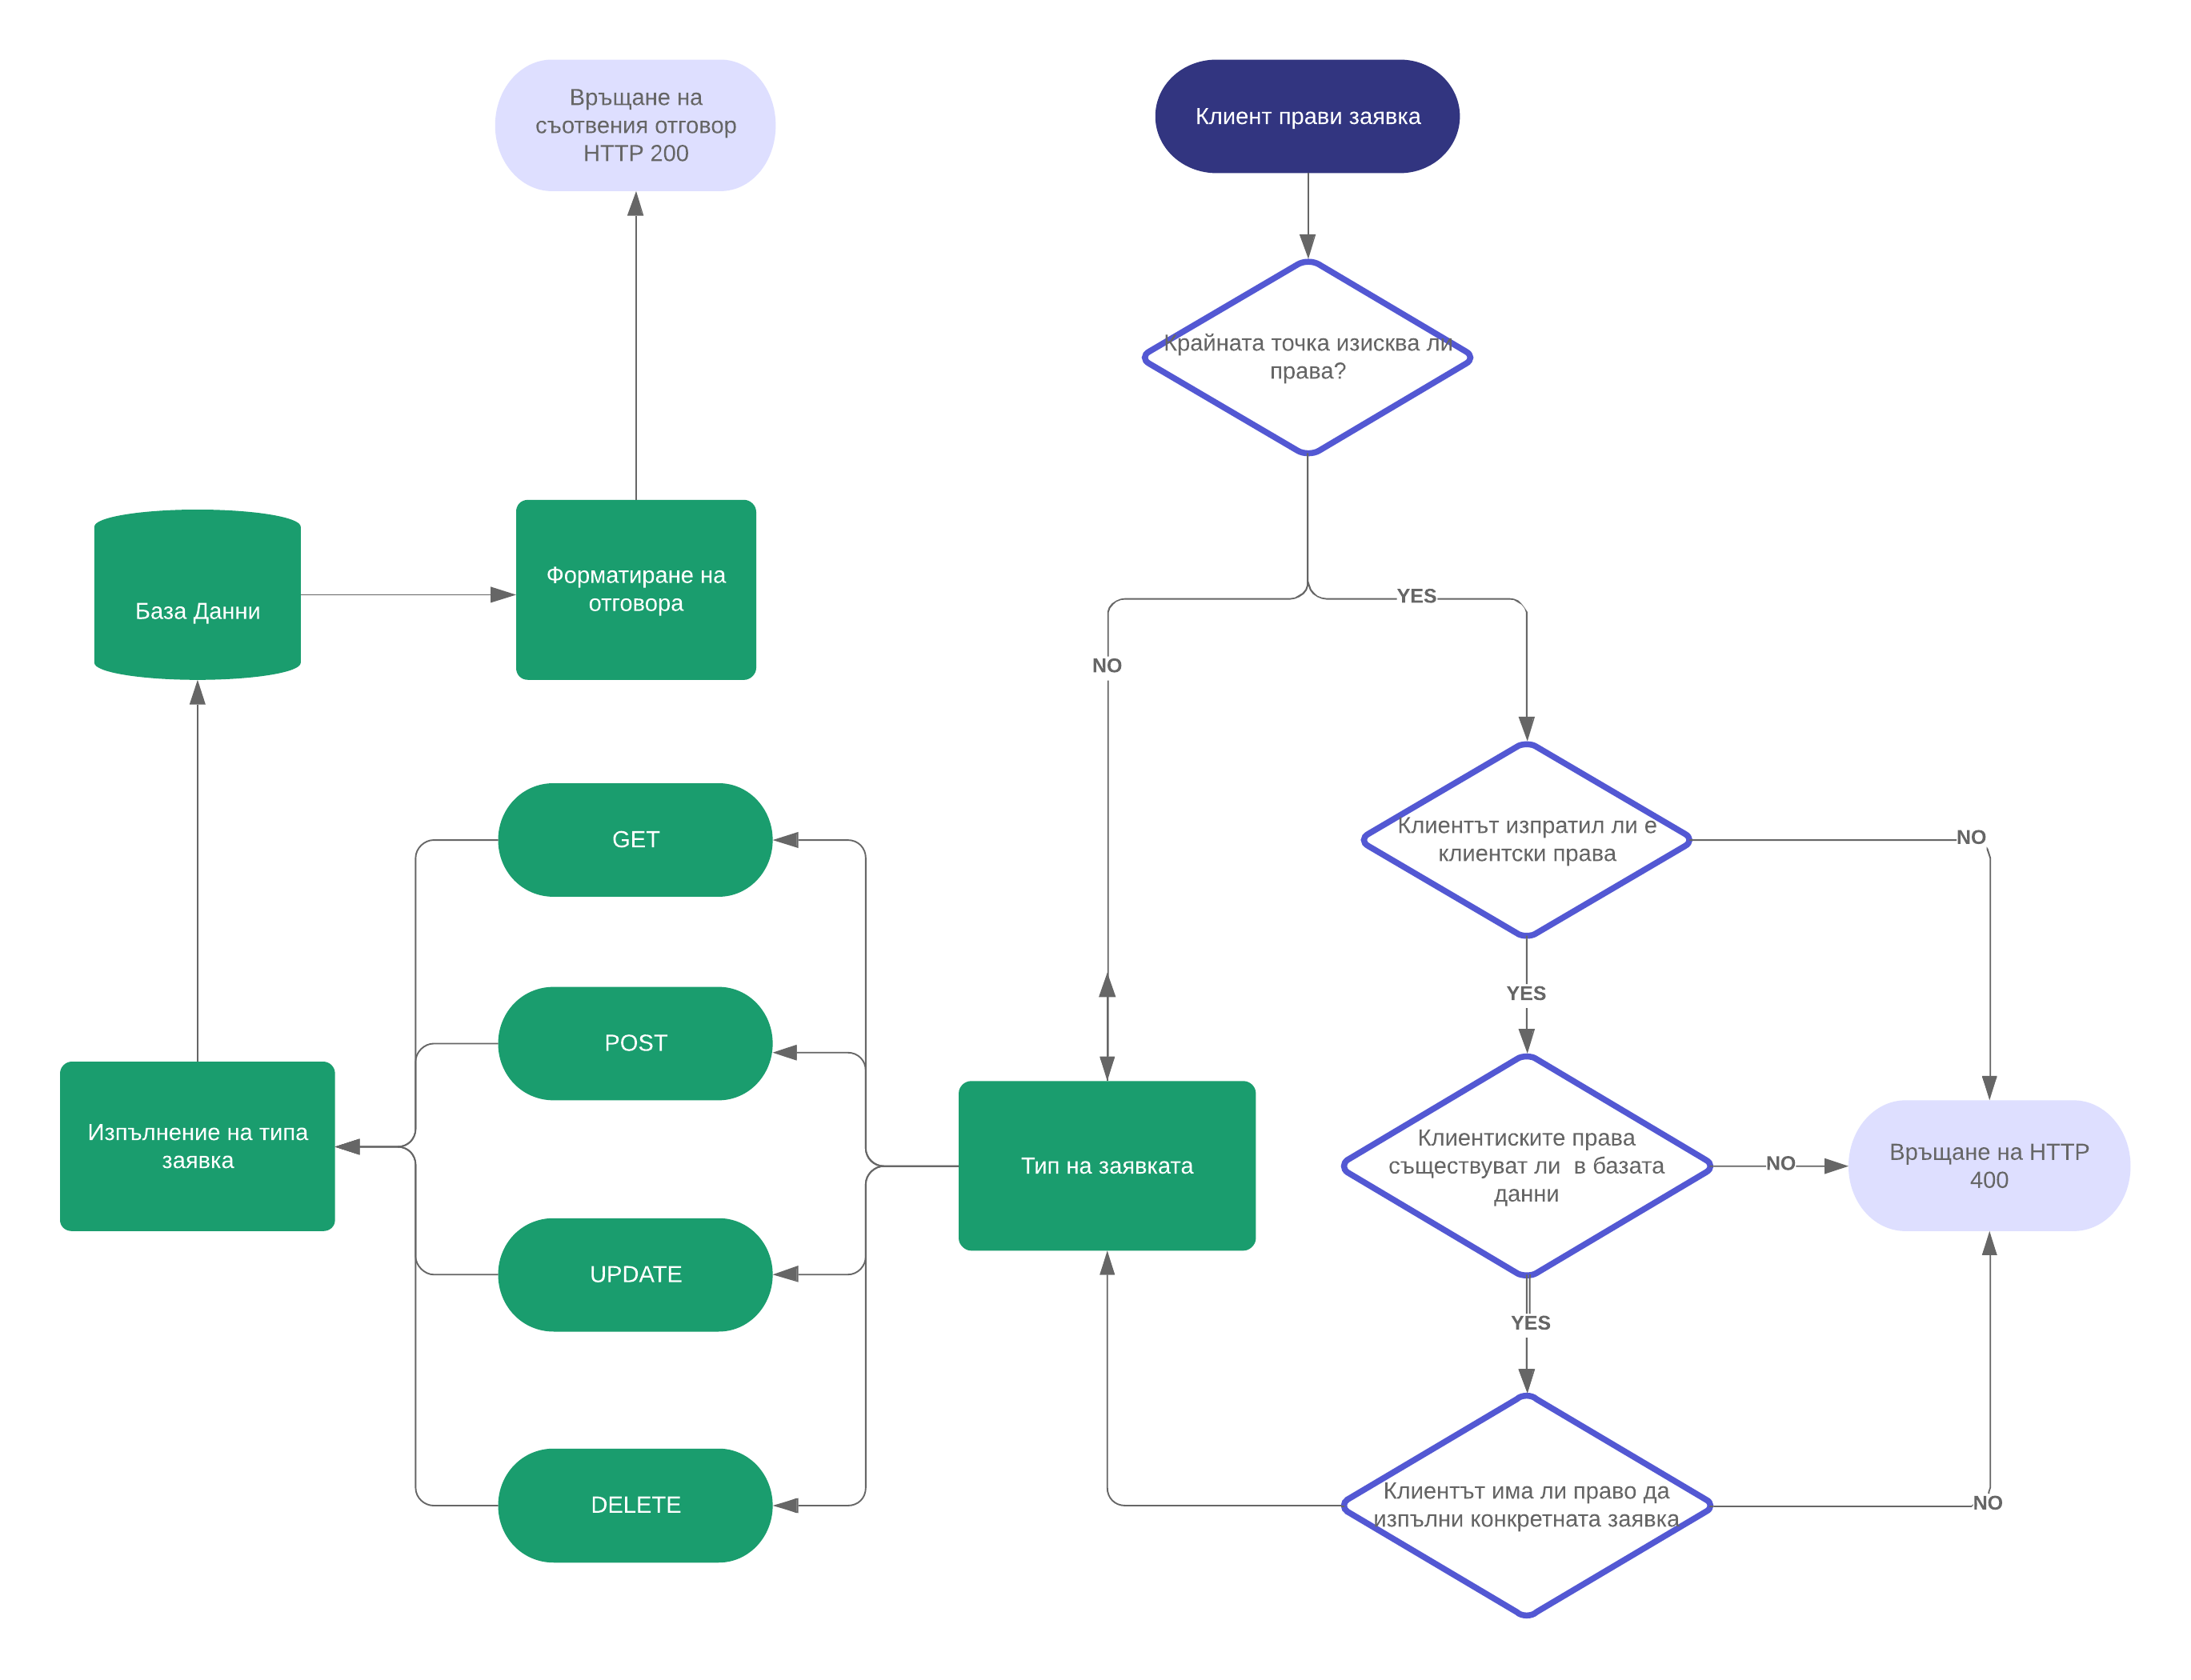
\includegraphics[width=1.2\textwidth]{images/Algorythm.png}}%
    \caption{Основен алгоритъм}
    \label{fig:app_algorythm}
\end{figure}

При изпълняване на заявка алгоритъмът на приложението първо проверява дали крайната точка изисква наличието на права. Ако тя изисква права се проверява дали клиентът има нужните права за изпълнението на заявката. Тъй като не може всеки клиент да прави промени по ресурси, които не му принадлежат, се правят проверки за собствеността на ресурсите, които клиентът желае да манипулира. Заявката се изпълнява ако клиентът, който я създава, съвпада със собственика на ресурсите. Алгоритъмът е показан и с блок схема на фигура \ref{fig:app_algorythm}.

\section{База данни}
\begin{figure}[h]
    \centering
    
\includegraphics{images/postgreSQL.png}
    \caption{PostgreSQL Лого}
    \label{fig:postgre_logo}
\end{figure}

Базата данни, която е използвана за проекта е PostgreSQL. Причината за този избор е, че PostgreSQL е релационна база данни. В проекта има много връзки между различните модели, които са създадени. Поради тази причина NoSQL база данни като MongoDB не би била добър избор. Специфицирайки връзките между различните модели можем да изберем и действията, които да се извършват при манипулация на свързаните към тях модели. При изтриване на User е желателно да се изтрият и Task-овете, които са създадени от него. PostgreSQL e перфектният избор за тази цел.

\begin{figure}[h]
    \centering
    \makebox[\textwidth][c]{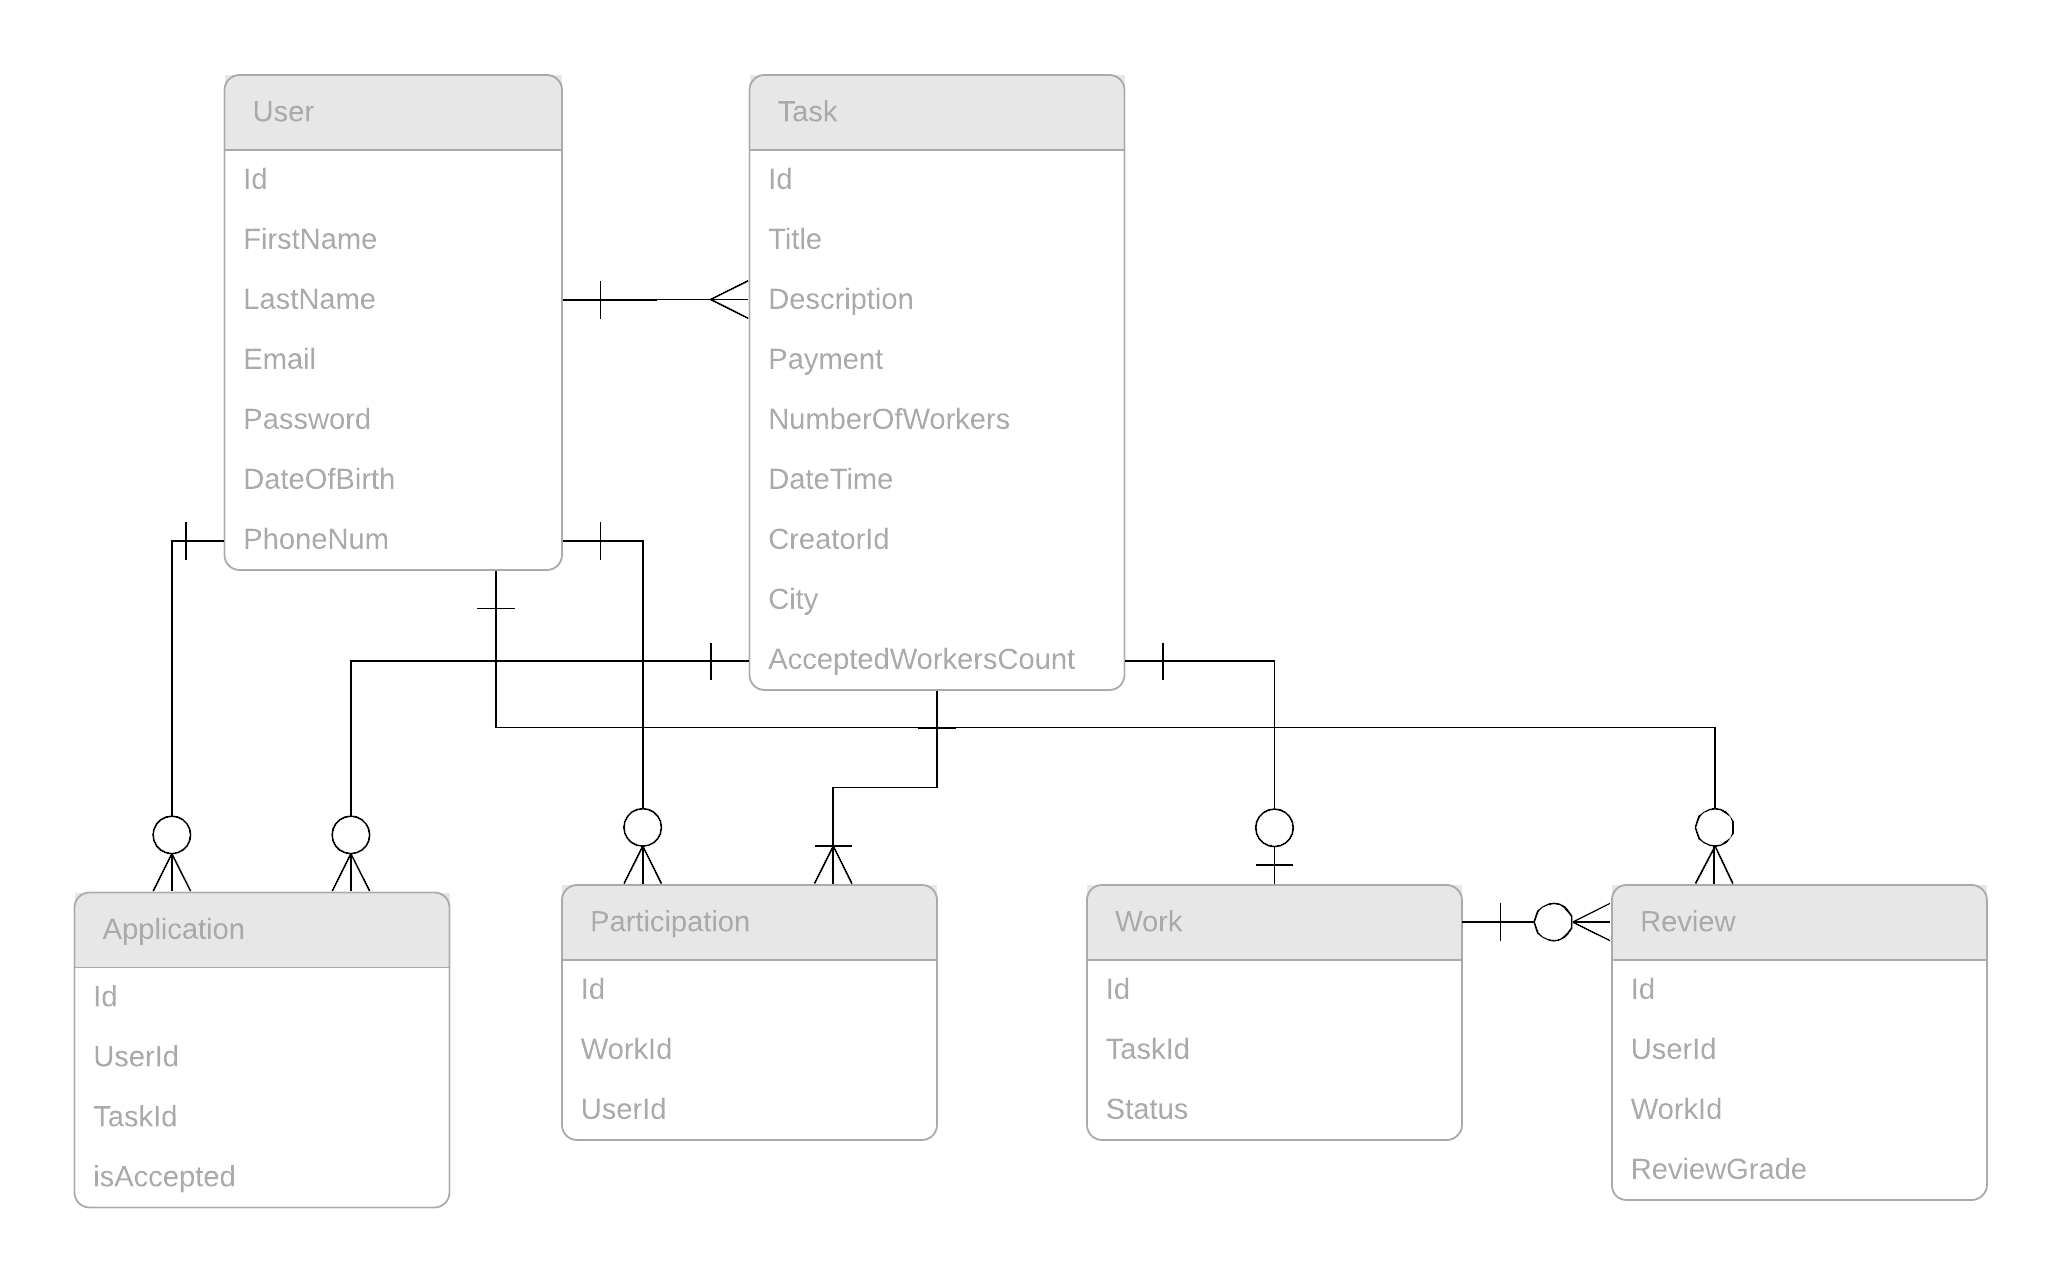
\includegraphics[width=1.2\textwidth]{images/Database.png}}%
    \caption{Схема на базата данни}
    \label{fig:database_schema}
\end{figure}

\newpage

На фигура \ref{fig:database_schema} са показани всичките таблици и връзките между тях. Показаните таблици са:

\begin{itemize}
    \item User - Информацията за потребителя
    \item Task - Обява за работа
    \item Application - Заявление за участие в конкретна работа
    \item Work - Започната работа
    \item Participation - Участие на конкретен потребител в конкретна започната работа
    \item Review - Обратна връзка от работодател към работник, оценка на работника за някоя работа
\end{itemize}